\documentclass[Main.tex]{subfiles} 
\begin{document}
\begin{figure}[H]%[htbp]
\centering
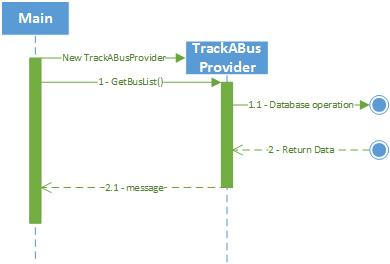
\includegraphics[scale=1.00]{Diagrammer/MainTrackABusThreadCom.jpg}
\caption{Sekvensdiagram over - Main og TrackABusProvider p� mobil applikationen}
\label{fig:SekvensdiagramTrackAbusThread}
\end{figure}
P� figur \ref{fig:SekvensdiagramTrackAbusThread} viser et eksemple p� hvordan main tr�den i mobil applikationen kommuniker med TrackABusProvideren. Det kan ses at main tr�den skaber en ny TrackABusProvider klasse, efter den er oprette er det muligt at kalde ned i den, dette vil skabe en ny tr�d der kalder ned i Data access layer for at hente data fra MySQL databasen, alt efter hvilken TrackABusProvider funktion der er blevet kaldet. Det kan ses at main tr�den ikke bliver blokeret imens der hentes fra databasen. N�r TrackABusProvider er f�rdig med at hente data fra databasen, bliver der sendt en besked, med det hentet data, til main tr�den, der nu vil, ved hj�lp af en message handler, pr�sentere det hentede data til brugeren.\\
UpdateTimeThread virker p� samme m�de, ved at main tr�den starter UpdateTimeThread n�r brugeren trykker p� et stoppested, tr�den vil nu k�re indtil at brugeren v�lger et nyt stoppsted, hvorved tr�den bliver lukket, og en ny UpdateTimeThread vil blive starten som hente tiden til det nye stoppested. tr�den vil ogs� blive stoppet ved at brugeren naviger v�k fra BusMapActivity'en.\\
SetFavoriteBusRoute og RemoveFavorite bliver blot startet af main tr�den, og sender en besked tilbage n�r de er f�rdige med at gemme eller slette fra SQLite databasen. Det vil ikke v�re muligt at starte en ny SetFavoriteBusRoute eller RemoveFavorite imens 1 af dem k�re.
\end{document}